\subsection{Расчет траектории полета}

В данном разделе была рассчитана траектория полета самолета-прототипа
Concorde. Траектория полета включает в себя следующие участки: набор высоты,
крейсерский полет, снижение. Ниже приведены формулы и соотношения,
которые были использованы при расчете

\subsubsection{Расчётные формулы и соотношения}
\label{sec:Расчётные формулы и соотношения}

\begin{center}
    Набор высоты:
\end{center}

Программа набора высоты, 1/с -- 
\begin{equation}
\label{eq:Программа набора}
    V' = \frac{dV}{dt} = \frac{V^{i+1}+V^{i}}{H^{i+1}+H^{i}}
\end{equation}

Коэффициент, используемый для расчета характеристик набора и снижения --  
\begin{equation}
    \label{eq:Коэффициент}
    \kappa = \frac{1}{\frac{V'V}{g}+1}
\end{equation}

Тангенциальная перегрузка --  
\begin{equation}
    \label{eq:Тангенциальная перегрузка }
    n_x = \frac{P\text{р}-P\text{п}}{mg}
\end{equation}

Угол набора высоты, град -- 
\begin{equation}
    \label{eq:Угол набора высоты}
    \theta_\text{наб} = n_x \cdot \kappa \cdot \frac{180^0}{\pi}
\end{equation}

Энергетическая скороподъемность, м/c -- 
\begin{equation}
    \label{eq:Энергетическая скороподъемность}
    V_y^* = V \cdot n_x
\end{equation}

Вертикальная скорость на участке набора высоты, м/с
\begin{equation}
    \label{eq:Вертикальная скорость на участке набора высоты}
    V_{y_\text{наб}} = V_y^* \cdot \kappa
\end{equation}

Дальность участка набора высоты, км -- 
\begin{equation}
    \label{eq:Дальность участка набора высоты}
    L_\text{наб} = \int_{H_\text{эк}}^{H_\text{эн}}\frac{dH_\text{э}}{1000 n_x}
\end{equation}

Время участка набора высоты, мин -- 
\begin{equation}
    \label{eq:Время участка набора высоты}
    t_\text{наб} = \int_{H_\text{эк}}^{H_\text{эн}}\frac{dH_\text{э}}{V_y^* 60}
\end{equation}

Масса топлива, расходуемого за участок набора, кг -- 
\begin{equation}
    \label{eq:Масса топлива, расходуемого за участок набора}
    m_T{_\text{наб}} = \int_{H_\text{эк}}^{H_\text{эн}}\frac{dH_\text{э}}{3600} \cdot \frac{C_eP_\text{р}}{V_y^*}
\end{equation}

\begin{center}
    Крейсерский полёт:
\end{center}

Относительный расход топлива -- 
\begin{equation}
    \label{eq:Относительный расход топлива}
    \bar{m}_{T_\text{кр}} = 1-\bar{m}_\text{сн}-\bar{m}_\text{цн} - \bar{m}_{T_\text{наб}} - \bar{m}_{T_\text{снп}} - \bar{m}_{T_\text{анз}} - \bar{m}_{T_\text{пр}}
\end{equation}

Время крейсерского полёта, мин -- 
\begin{equation}
    \label{eq:Время крейсерского полёта}
    T_\text{кр} = \frac{60 K_\text{ГП}}{g \cdot C_e} \ln{\frac{1 - \bar{m}_{T_\text{наб}} - \bar{m}_{T_\text{пр}}}{1 - \bar{m}_{T_\text{кр}} - \bar{m}_{T_\text{наб}} - \bar{m}_{T_\text{пр}}}}
\end{equation}

Дальность крейсерского полёта, км -- 
\begin{equation}
    \label{eq:Дальность крейсерского полёта}
    L_\text{кр} = \frac{3,6 V K_\text{ГП}}{g \cdot C_e} \ln{\frac{1 - \bar{m}_{T_\text{наб}} - \bar{m}_{T_\text{пр}}}{1 - \bar{m}_{T_\text{кр}} - \bar{m}_{T_\text{наб}} - \bar{m}_{T_\text{пр}}}}
\end{equation}

Плотность воздуха на высоте, кг/м$^3$
\begin{equation}
    \label{eq:Плотность воздуха на высоте}
    \rho_\text{нкр} = \frac{2 \bar{m}_\text{ккр}Ps10}{C_{y_\text{ГП}}V_\text{к}^2}
\end{equation}

\begin{center}
    Снижение:
\end{center}

Дальность участка снижения высоты, км -- 
\begin{equation}
    \label{eq:Дальность участка снижения высоты}
    L_\text{сн} = \int_{H_\text{эк}}^{H_\text{эн}}\frac{dH_\text{э}}{1000 n_x}
\end{equation}

Время участка снижения высоты, мин -- 
\begin{equation}
    \label{eq:Время участка снижения высоты}
    t_\text{сн} = \int_{H_\text{эк}}^{H_\text{эн}}\frac{dH_\text{э}}{V_y^* 60}
\end{equation}

Масса топлива, расходуемого за участок снижения, кг -- 
\begin{equation}
    \label{eq:Масса топлива, расходуемого за участок снижения}
    m_T{_\text{сн}} = \int_{H_\text{эк}}^{H_\text{эн}}\frac{dH_\text{э}}{3600} \cdot \frac{C_eP_\text{р}}{V_y^*}
\end{equation}

\subsubsection{Расчет характеристик набора высоты}

В начале расчета необходимо определить H, М в начале набора высоты и
H, М в конце набора высоты.

Начальные значения H и М определяются следующим образом $H_0 = 0 $ км $M_0 = 1,2 \cdot M_{min \text{доп}}$,а конечные значения выбираются из условия минимума километрового расхода топлива в установившемся горизонтальном полете. Высота и число Маха, при которых километровый расход топлива принимает наименьшее значение, определены в предыдущем разделе (см. раздел \ref{sec:Результаты расчета летно-технических характеристик
самолета-прототипа Concorde},таблица \ref{tab:Основные ограничения на область полётов}) 

При наборе высоты режим работы двигателя - "максимал". 

Учитывая сказанное выше, получаем:
\begin{itemize}
    \item [-] Начало набора высоты: $H_0 = 0$ км, $M_0 = 1,2 \cdot 0,276 = 0,3312$
    \item [-] Окончание набора высоты: $H_\text{к} = 10,8$ км, $M_\text{к} = 0,8$
\end{itemize}

В качестве программы принимается полученная в разделе \ref{sec:Результаты расчета летно-технических характеристик самолета-прототипа Concorde} зависимость $M_\text{наб}(M)$ соответствующая максимальной энергетической скороподъемности. Данная программа близка к оптимальным программам набора высоты по критериям минимума расхода топлива или набора времени. 

Зная программу набора высоты можно найти её характеристики: угол наклона траектории $\theta_\text{наб}$, вертикальная скорость $V_{y_\text{наб}}$, время $t_\text{наб}$ , дальность $L_\text{наб}$, расход топлива $M_{T_\text{наб}}$, они определяются по формулам \ref{eq:Программа набора}-\ref{eq:Масса топлива, расходуемого за участок набора}. Результаты расчетов характеристик набора высоты оформлены в виде таблицы (см.таблицу \ref{tab:Результаты расчета характеристик набора высоты}) 

\begin{longtable}[H]{|c|c|c|c|c|c|c|c|}
    \caption{Результаты расчета характеристик набора высоты} \label{tab:Результаты расчета характеристик набора высоты} \\
    \hline 
    H, м& $M$ & $V$, м/с & $n_x$ & $V_y^*$, м/c & $H_\text{э}$, м & $C_e$, кг/($H \cdot$ ч) & $P_\text{п}$\\ \hline
    \endfirsthead
    
    \multicolumn{8}{c}%
    {{ \tablename\ \thetable{}: Результаты расчета характеристик набора высоты}} \\
    \hline 
    H, км& $M$ & $V$, м/с & $n_x$ & $V_y^*$, м/c & $H_\text{э}$ &, м $C_e$, кг/($H \cdot$ ч) & $P_\text{п}$\\ \hline
    \endhead
    \endfoot
    
    \hline \hline
    \endlastfoot
    \hline
    0 & 0.33 & 112.74 & 0.3 & 34.0 & 647.83 & 0.9399 & 74133.0 \\ \hline 1000 & 0.37 & 124.71 & 0.28 & 34.53 & 1792.64 & 0.9365 & 77157.0 \\ \hline 2000 & 0.4 & 133.75 & 0.25 & 33.57 & 2911.71 & 0.9306 & 78395.0 \\ \hline 3000 & 0.43 & 140.73 & 0.23 & 31.75 & 4009.48 & 0.9234 & 78396.0 \\ \hline 4000 & 0.45 & 147.41 & 0.2 & 29.75 & 5107.59 & 0.916 & 77976.0 \\ \hline 5000 & 0.48 & 154.9 & 0.18 & 27.98 & 6223.01 & 0.9095 & 77670.0 \\ \hline 6000 & 0.52 & 163.05 & 0.16 & 26.6 & 7354.99 & 0.904 & 77382.0 \\ \hline 7000 & 0.55 & 171.59 & 0.15 & 25.59 & 8500.7 & 0.8996 & 76984.0 \\ \hline 8000 & 0.59 & 180.91 & 0.14 & 24.71 & 9668.18 & 0.8959 & 76588.0 \\ \hline 9000 & 0.63 & 191.09 & 0.12 & 23.51 & 10861.06 & 0.8921 & 76216.0 \\ \hline 10000 & 0.67 & 201.03 & 0.11 & 21.62 & 12059.82 & 0.8874 & 75512.0 \\ \hline 11000 & 0.71 & 209.3 & 0.1 & 20.07 & 13232.68 & 0.8853 & 74205.0
    
        
\end{longtable}


\begin{longtable}[H]{|c|c|c|c|c|c|c|}
    \caption{Результаты расчета характеристик набора высоты} \label{tab:Результаты расчета характеристик набора высоты} \\
    \hline 
    H, м & $V'$, 1/с & $\theta_\text{наб}$, град& $V_{y_\text{наб}}$, м/c& $\Delta H_\text{э}$, м& $1/n_{x_\text{ср}}$&$1/V^*_{y_\text{наб}}$, c/м\\ \hline
    \endfirsthead
    
    \multicolumn{6}{c}%
    {{ \tablename\ \thetable{}: Результаты расчета характеристик набора высоты}} \\
    \hline 
    H, м & $V'$, 1/с & $\theta_\text{наб}$, град& $V_{y_\text{наб}}$, м/c& $\Delta H_\text{э}$, м& $1/n_{x_\text{ср}}$&$1/V^*_{y_\text{наб}}$, c/м\\ \hline
    \endhead
    \endfoot
    
    \hline \hline
    \endlastfoot
    \hline
    0 & 0.012 & 15.19 & 29.9 & 1144.7 & 3.464 & 0.03 \\ \hline 1000 & 0.0091 & 14.23 & 30.96 & 1119.2 & 3.798 & 0.03 \\ \hline 2000 & 0.007 & 13.13 & 30.64 & 1097.9 & 4.209 & 0.03 \\ \hline 3000 & 0.0067 & 11.8 & 28.98 & 1097.9 & 4.695 & 0.03 \\ \hline 4000 & 0.0075 & 10.4 & 26.75 & 1114.9 & 5.246 & 0.03 \\ \hline 5000 & 0.0082 & 9.17 & 24.78 & 1132.5 & 5.833 & 0.04 \\ \hline 6000 & 0.0087 & 8.17 & 23.25 & 1147.9 & 6.418 & 0.04 \\ \hline 7000 & 0.0092 & 7.36 & 22.06 & 1165.3 & 7.014 & 0.04 \\ \hline 8000 & 0.0097 & 6.64 & 20.95 & 1184.1 & 7.725 & 0.04 \\ \hline 9000 & 0.0104 & 5.86 & 19.51 & 1207.5 & 8.713 & 0.04 \\ \hline 10000 & 0.011 & 5.03 & 17.64 & 1231.5 & 9.849 & 0.05 \\ \hline 11000 & 0.0147 & 4.18 & 15.48 & 1328.4 & 11.881 & 0.05 \\ \hline 12000 & 0.0153 & 3.17 & 12.54 & 1364.3 & 14.714 & 0.06 \\ \hline 13000 & 0.0166 & 2.53 & 10.68 & 1424.3 & 17.624 & 0.07 \\ \hline 14000 & 0.0186 & 2.0 & 9.05 & 1507.5 & 21.65 & 0.08 \\ \hline 15000 & 0.0192 & 1.54 & 7.45 & 1561.3 & 28.284 & 0.1 \\ \hline 16000 & 0.018 & 1.14 & 5.91 & 1560.6 & 40.05 & 0.13
    
\end{longtable}

\begin{figure}[H]
    \center{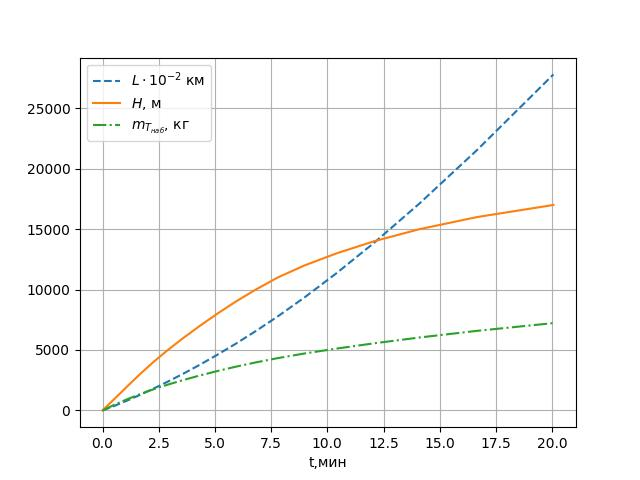
\includegraphics[width=\linewidth]{Оглавление/Part1/figures/Характеристики набора высоты1.jpg}}
    \caption{Характеристики набора высоты}
    \label{fig:Характеристики набора высоты1}
\end{figure}

\begin{figure}[H]
    \center{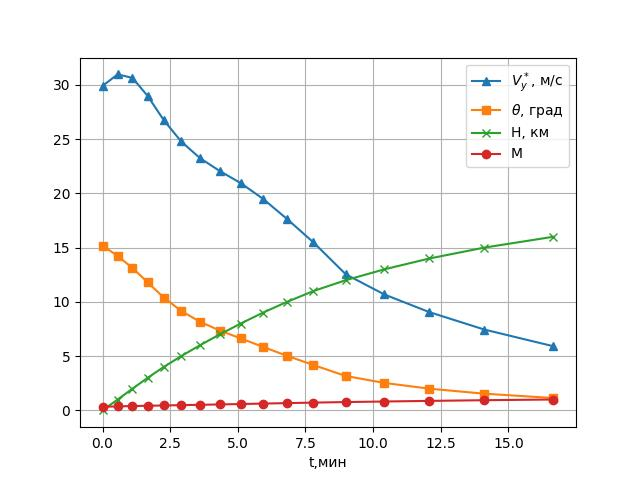
\includegraphics[width=\linewidth]{Оглавление/Part1/figures/Характеристики набора высоты2.jpg}}
    \caption{Характеристики набора высоты}
    \label{fig:Характеристики набора высоты2}
\end{figure}

\begin{table}[H]
    \centering
    \caption{Конечные результаты расчета параметров набора}
    \begin{tabular}{|c|c|}
    \hline
        Параметр & Значение \\ \hline
        $m_{T_\text{наб}}$ & 4310,3 кг\\ \hline
        $L_\text{кр}$ & 77,2 км\\ \hline
        $T_\text{кр}$ & 13,63 мин\\ \hline
    \end{tabular}
    \label{tab:Крейсер}
\end{table}


\subsubsection{Расчет характеристик крейсерского полета}
\label{sec: Расчет характеристик крейсерского полета}

В данном подразделе необходимо определить дальность и
продолжительность крейсерского полета, последовательность расчетов
изложена далее.
Относительный расход топлива на участке крейсерского полета вычисляется
при максимальной целевой (полезной) нагрузке для неманевренного самолета
по формуле \ref{eq:Относительная масса пустого снаряженного самолета}: 

\begin{equation}
    \label{eq:Относительная масса пустого снаряженного самолета}
    \bar{m}_{T_\text{кр}} = 1 - \bar{m}_{\text{цн}} - \bar{m}_{T_\text{наб}} - \bar{m}_{T_\text{снп}} - \bar{m}_{T_\text{анз}} - \bar{m}_{T_\text{пр}}
\end{equation}
$\bar{m}_{T_\text{сн}} = 0,5$ -- относительная масса пустого снаряженного самолета \\ 
$\bar{m}_{\text{цн}} = 0,15$ -- относительная масса целевой нагрузки \\ 
$\bar{m}_{T_\text{снп}} = 0,015$ -- относительная масса топлива, расходуемая при снижении и
посадке \\ 
$\bar{m}_{T_\text{наб}}$ --  относительная масса топлива,
расходуемая при наборе высоты \\

Используя формулы из раздела \ref{sec:Расчётные формулы и соотношения} расчитаем: 

\begin{itemize}
    \item [-] высоту конца крейсерского полёта $H_{\text{к} \ \text{кр}}$
    \item [-] дальность крейсерского полёта $L_\text{кр}$
    \item [-] продолжительность полёта $T_\text{кр}$
\end{itemize}
Все данные приведены в таблице (\ref{tab:Крейсер})

\begin{table}[H]
    \centering
    \caption{Конечные результаты расчетов}
    \begin{tabular}{|c|c|}
    \hline
        Параметр & Значение \\ \hline
        $H_{\text{к} \ \text{кр}}$ & 12,300 км\\ \hline
        $L_\text{кр}$ & 5910 кг\\ \hline
        $T_\text{кр}$ & 470 мин\\ \hline
    \end{tabular}
    \label{tab:Крейсер}
\end{table}


\subsubsection{Расчет характеристик снижения}

В данном подразделе производится расчет следующих характеристик
снижения: угол наклона траектории $\theta_\text{сн}$, вертикальная скорость $V_{y_\text{сн}}$, время $t_\text{сн}$ ,дальность $L_\text{сн}$. Расчет проводится по формулам \ref{eq:Дальность участка снижения высоты}-\ref{eq:Масса топлива, расходуемого за участок снижения}, аналогичным расчету участка набора высоты. 

В качестве программы снижения принимается полученная в разделе \ref{sec:Результаты расчета летно-технических характеристик самолета-прототипа Concorde} зависимость $M_\text{сн}(H)$, соответствующая минимуму потребной тяги (максимальному аэродинамическому качеству). Данная программа близка к оптимальной программе снижения с точки зрения получения максимальной дальности полета. 
Программа снижения содержит два участка:
\begin{enumerate}
    \item торможение на высоте $H_\text{кр}$ до скорости $M(P_{\text{п} \ min})$
    \item снижение до высоты $H = 0$ км
\end{enumerate} 

При снижении режим работы двигателя - "малый газ". 

Высота начала снижения равна высоте полета самолета в конце крейсерского участка ($H_{0_\text{кр}} = H_\text{к \ кр}$) Число $M$(скорость $V$[км/ч]) полета соответствует минимуму потребной тяги на высоте $H_{0_\text{сн}}$, определяется по графику $M(P_{\text{п} \ min})$, построенному в разделе \ref{sec:Результаты расчета летно-технических характеристик самолета-прототипа Concorde}

Высота конца участка снижения условно принимается равной нулю ($H_\text{к \ сн}$). Скорость в конце снижения соответствует наивыгоднейшей скорости при $H = 0$ км, $M_\text{ксн}(P_{\text{п} \ min})$.  Исходя из вышесказанного, получим:
\begin{itemize}
    \item [-] Начальные условия: $H_{0 \ \text{сн}} = 11$ км, $M_{0 \ \text{сн}} 0,$
    \item [-] Конечные условия: $H_{\text{к} \ \text{сн}} = 0$ км, $M_{\text{к} \ \text{сн}}$
\end{itemize}

Все рассчитанные характеристики снижения занесены в таблицу \ref{tab: } 

\begin{longtable}[H]{|c|c|c|c|c|c|c|c|}
    \caption{Результаты расчета характеристик набора высоты} \label{tab:Результаты расчета характеристик набора высоты} \\
    \hline 
    H, м& $M$ & $V$, м/с & $n_x$ & $V_y^*$, м/c & $H_\text{э}$, м & $C_e$, кг/($H \cdot$ ч) & $P_\text{п}$\\ \hline
    \endfirsthead
    
    \multicolumn{8}{c}%
    {{ \tablename\ \thetable{}: Результаты расчета характеристик набора высоты}} \\
    \hline 
    H, км& $M$ & $V$, м/с & $n_x$ & $V_y^*$, м/c & $H_\text{э}$ &, м $C_e$, кг/($H \cdot$ ч) & $P_\text{п}$\\ \hline
    \endhead
    \endfoot
    
    \hline \hline
    \endlastfoot
    \hline
    11& 0.58 & 172.4 & -0.04 & -6.81 & 12514.81 & 0.1701 & 3325.0 \\ \hline 10 & 0.55 & 164.48 & -0.04 & -6.48 & 11378.89 & 0.1708 & 3649.0 \\ \hline 9 & 0.51 & 155.14 & -0.04 & -6.08 & 10226.69 & 0.1721 & 4070.0 \\ \hline 8 & 0.47 & 145.78 & -0.04 & -5.69 & 9083.15 & 0.1733 & 4457.0 \\ \hline 7 & 0.44 & 137.43 & -0.04 & -5.34 & 7962.63 & 0.1744 & 4826.0 \\ \hline 6 & 0.41 & 129.81 & -0.04 & -5.01 & 6858.8 & 0.1756 & 5239.0 \\ \hline 5 & 0.38 & 122.38 & -0.04 & -4.69 & 5763.35 & 0.177 & 5758.0 \\ \hline 4 & 0.36 & 115.59 & -0.04 & -4.39 & 4681.03 & 0.1785 & 6379.0 \\ \hline 3 & 0.33 & 109.97 & -0.04 & -4.13 & 3616.34 & 0.1803 & 7057.0 \\ \hline 2 & 0.32 & 105.13 & -0.04 & -3.91 & 2563.35 & 0.1821 & 7738.0 \\ \hline 1 & 0.3 & 100.28 & -0.04 & -3.69 & 1512.54 & 0.184 & 8368.0 \\ \hline 0 & 0.28 & 95.31 & -0.04 & -3.48 & 463.02 & 0.1857 & 8892.0
    
        
\end{longtable}


\begin{longtable}[H]{|c|c|c|c|c|c|c|}
    \caption{Результаты расчета характеристик набора высоты} \label{tab:Результаты расчета характеристик набора высоты} \\
    \hline 
    H, м & $V'$, 1/с & $\theta_\text{спуск}$, град& $V_{y_\text{спуск}}$, м/c& $\Delta H_\text{э}$, м& $1/n_{x_\text{ср}}$&$1/V^*_{y_\text{спуск}}$, c/м\\ \hline
    \endfirsthead
    
    \multicolumn{6}{c}%
    {{ \tablename\ \thetable{}: Результаты расчета характеристик набора высоты}} \\
    \hline 
    H, м & $V'$, 1/с & $\theta_\text{спуск}$, град& $V_{y_\text{спуск}}$, м/c& $\Delta H_\text{э}$, м& $1/n_{x_\text{ср}}$&$1/V^*_{y_\text{спуск}}$, c/м\\ \hline
    \endhead
    \endfoot
    
    \hline \hline
    \endlastfoot
    \hline
    11-10 & 0.0079 & -1.99 & -5.98 & -1135.9 & -25.347 & -0.15 \\ \hline 10-9 & 0.0093 & -1.95 & -5.6 & -1152.2 & -25.449 & -0.16 \\ \hline 9-8 & 0.0094 & -1.96 & -5.3 & -1143.5 & -25.567 & -0.17 \\ \hline 8-7 & 0.0083 & -1.99 & -5.06 & -1120.5 & -25.685 & -0.18 \\ \hline 7-6 & 0.0076 & -2.01 & -4.82 & -1103.8 & -25.817 & -0.19 \\ \hline 6-5 & 0.0074 & -2.02 & -4.57 & -1095.4 & -25.985 & -0.21 \\ \hline 5-4 & 0.0068 & -2.03 & -4.33 & -1082.3 & -26.201 & -0.22 \\ \hline 4000 & 0.0056 & -2.04 & -4.12 & -1064.7 & -26.458 & -0.23 \\ \hline 3-2 & 0.0048 & -2.04 & -3.92 & -1053.0 & -26.739 & -0.25 \\ \hline 2-1 & 0.0049 & -2.03 & -3.72 & -1050.8 & -27.016 & -0.26 \\ \hline 1-0 & 0.005 & -2.01 & -3.52 & -1049.5 & -27.264 & -0.28
    
\end{longtable}

\begin{figure}[H]
    \center{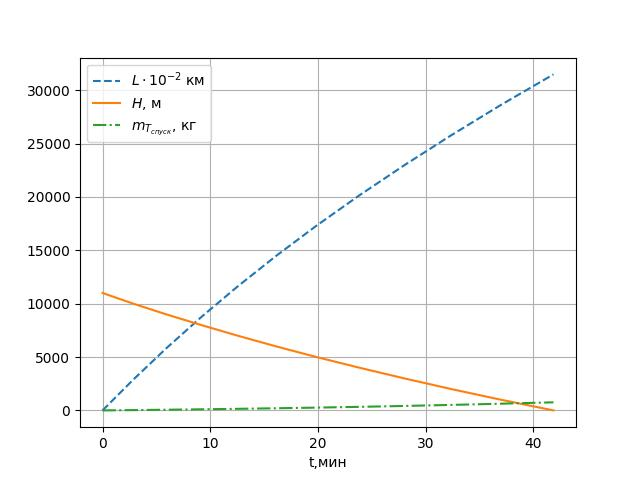
\includegraphics[width=\linewidth]{Оглавление/Part1/figures/Характеристики Спуска1.jpg}}
    \caption{Характеристики снижения}
    \label{fig:Характеристики Спуска1}
\end{figure}

\begin{figure}[H]
    \center{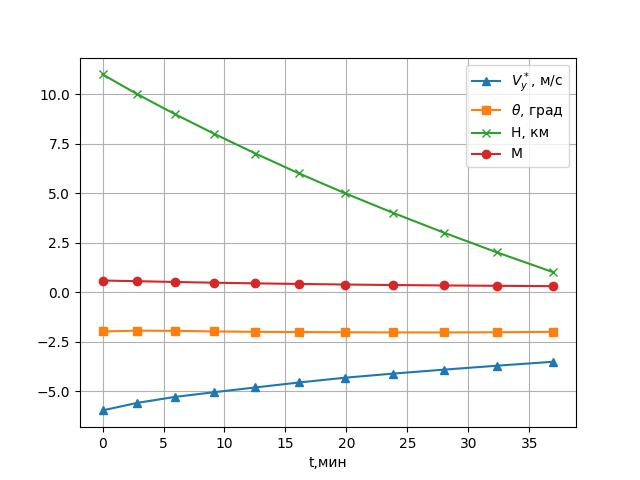
\includegraphics[width=\linewidth]{Оглавление/Part1/figures/Характеристики пуска2.jpg}}
    \caption{Характеристики снижения}
    \label{fig:Характеристики Спуска2}
\end{figure}

\begin{table}[H]
    \centering
    \caption{Конечные результаты расчета параметров набора}
    \begin{tabular}{|c|c|}
    \hline
        Параметр & Значение \\ \hline
        $m_{T_\text{наб}}$ & 757 кг\\ \hline
        $L_\text{кр}$ & 314,78 км\\ \hline
        $T_\text{кр}$ & 41,866 мин\\ \hline
    \end{tabular}
    \label{tab:Крейсер}
\end{table}

Зная, дальность набора высоты, крейсерского полета, снижения, высоту крейсерского полета, высоту конца крейсерского полета, рассчитанную траекторию полета можно представить графически (см. рис.\ref{fig:Траектория полёта}) 


\begin{figure}[H]
    \center{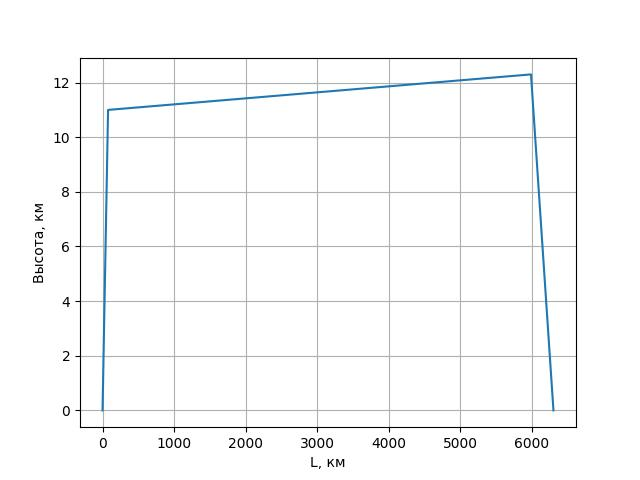
\includegraphics[width=\linewidth]{Оглавление/Part1/figures/Траектория полета.jpg}}
    \caption{Траектория полёта}
    \label{fig:Траектория полёта}
\end{figure}

Общая дальность полета и общая продолжительность полета равны:
\begin{itemize}
    \item [-] $L = 77,2 \text{ км} + 5909,75 \text{ км} + 314км = 6300\text{ км}$
    \item [-] $T = 12,3 \text{ мин} + 470,1 \text{ мин} + 41,86 \text{ мин} = 524,26 \text{ мин}$
\end{itemize}

\begin{center}
    Выводы:
\end{center}

После выполнения расчетов траектории полета самолета-прототипа Concorde
были получены следующие результаты:
\begin{itemize}
\item[-] общая дальность полета равна 6300 км
\item[-] общее время полета составляет 524,26 мин
\item[-] дальность набора высоты равна 77,2 км
\item[-] топливо, израсходованное на набор высоты равно 4310 кг
\item[-] время набора высоты равно 12,3 мин
\item[-] дальность снижения равна 314 км
\item[-] топливо, израсходованное на снижение равно 757 кг
\item[-] время снижения 41 мин
\end{itemize}
По вышеперечисленным результатам у данного самолета довольно большая
общая дальность полета, что позволяет ему совершать транспортировку
пассажиров на значительные расстояния 